\chapter{Predicting Stocks Using Sentiment Analysis - Felix} \label{ch:predictions_ml}
The value of stocks is affected by external events. But information that moves the markets is also captured for example in news articles, online posts on social media or detailed financial reports. One can try to exploit the information presented in the news before it is fully absorbed by the markets. To do so, text data is processed and sentiments are extracted to infer whether the text conveys rather positive or negative information (see \citet{HADDI201326}). Using this information one can either try to predict stocks directly or to forecast future volatility (see \citet{robertson2007news}). This chapter will explore ways to leverage information from news using machine learning to predict the movement of stocks. It will first extract sentiments from text data using two unsupervised learning methods. Secondly, these sentiments will be used for a binary classification of upwards or downwards movement of the ten stocks using XGBoost.

% später
%The news data would need to be as precise as possible, because \citet{gidofalvi2001using} mentions that an effect on the stocks can only be measured up to 20min after the news appear. 
%In a paper by \citet{atkins2018financial} they compare the prediction of stock movement and volatility forecasts using naïve Bayes classifiers. They conclude that movement predictions with 49 Percent accuracy are not successful. 
As we did not have access to good news data, we implemented our approach on the available analyst reports. In contrast to current news, the analyst reports are released much less frequently  and focus more on past performance of stocks than new information. As such they are not able to incorporate current events as quickly as the news. The reports also cluster around certain dates with long stretches of no or very few reports in between (Figure \ref{fig:Seasonality in the Reports}). This makes it unlikely that they are valuable for trading strategies.
\\ 
\section{Overview of Existing Methods for Sentiment Extraction}
There exist several methods to obtain sentiment scores from text data. Most commonly procedures rely on a library of previously known positive and negative words or groups of words called 4-grams. The simplest method, called bag-of-words methods, simply counts the number of positive and negative words in the text. Other approaches extract parts of the text around the location of specific words and then use Support Vector Machines or Naive Bayes Classifier to generate sentiment scores (see \citet{westerski2007sentiment} for further references). Many of these more advanced sentiment classification techniques are supervised learning methods. As such they need a labelled data set for initial training. They are therefore not applicable to our 17153 analyst reports, because these are unstructured and not labelled. Also, the reports have a very specific format and language, therefore other pretrained models or other labelled training data sets could not be used. Other strategies for financial data rely on the availability of intra day trading and news data: By looking at the movement or volatility of the period close after the news release one can estimate approximate sentiment scores \citep{robertson2007news}. As the our stock data is only inter day we could not apply this method.
\\
\section{Sentiment Extraction - Theoretical Background}
Two methods to estimate sentiment scores in an unsupervised way will be explored here. The first one is a library-based approach, the second one is the so called Joint Sentiment Topic Model. 

\subsection{Sentiment Library Method}\label{BoW}
Our first method for extracting sentiments relies on a library that categorizes words as positive or negative. We can apply this library to the analyst report and obtain the number of positive (P) and the number of negative words (N) in the report. A sentiment or polarity score can then be calculated for each report from the relative frequencies of positive and negative words: 
\begin{equation}
    Polarity = \frac{P - N}{P + N}
\end{equation}\label{eq:polarity}
Some more advanced libraries even measure the positiveness of each word with a numeric score (and not only 1 and -1), but we could not find any library appropriate for our purposes. Instead we used a library from \citet{sent_dictionary} as simple word list. An excerpt from the list can be found in Table \ref{tab:sent_dic}. 
\begin{table}[ht]
\centering
\begin{tabular}{rll}
  \hline
 & positive & negative \\ 
 & $n = 218$ & $n = 1282$ \\ 
  \hline
  1 & acclaim & abandonment \\ 
  2 & accomplishment & abdication \\ 
  3 & advantage & abuse \\ 
  4 & assure & acquittal \\ 
  5 & attractiveness & catastrophe \\ 
  6 & delightful & criticize \\ 
  7 & diligent & degrade \\ 
  8 & impress & harsh \\ 
  9 & \vdots & \vdots \\ 
   \hline
\end{tabular}
\caption{Excerpt from the sentiment dictionary by 
\citet{sent_dictionary}}
\label{tab:sent_dic}
\end{table}

\subsection{Joint Sentiment Topic Model}\label{JST}
As a second method for extracting sentiments, we use the Joint Sentiment Topic Model by \citet{lin2009joint}. First, the user provides a number of topics to be estimated. Given the desired number of topics, the JST approach then automatically creates topics and assigns probabilities to the individual words of being associated to the different topics. Similar to, e.g. an exploratory factor analysis, one cannot always know why some words are grouped more closely together than others. The JST method heaviliy relies on the ideas of \citet{blei2003latent} and uses a Bayesian hierarchical model, called Latent Dirichlet Allocation (LDA) for the topic detection. JST, however, goes one step further by also assigning sentiment scores to words within specific topics. 

To better understand the procedure we will first have a closer look at LDA and then discuss the additional features of the JST. 
%For both approaches the text data has to be cleaned which is described in section \ref{cleaningText}, the subsequent analysis of the sentiment scores can be found in section \ref{BoW} and \ref{JST}.
The general idea of LDA is that each document can be described as coming from a distribution of topics. A financial report could for example be classified as being 50\% about politics, 30\% about environment and 20\% about the chemical industry. To be more precise however, the topics are not assigned explicit names or meanings by the model. The classification would therefore rather look like 50\% topic 1, 30\% topic 2 etc. Each topic can itself be described by a distribution of words \citep{blei2003latent} that indicates how likely a word is to appear in a specific topic. This assumes that the words themselves are independent of each other which is in reality not the case, but for large data sets this assumption seems to be acceptable. The LDA has two Dirichlet priors containing hyperparameters $\alpha$ and $\beta$. A high $\alpha$ indicates that each document is likely to contain a mixture of many topics, while a low $\alpha$ indicates that one document is strongly associated with one or few topics. Similarly a high $\beta$ implies that the words contained in each topic have a high overlap, while a low $\beta$ means that words are strongly associated with only one topic. LDA backtracks from the document level to identify topics that are likely to have generated this specific corpus of words. The underlying optimisation of the model is done using a Gibbs-Sampler. In the first step, each word is assigned a probability to belong to each of the $T$ topics. Those probabilities of course sum up to one. each document also gets a probability to contain each of the $T$ topics. The algorithm then iterates over the words, topics and documents, updating the underlying probabilities. In the Joint Sentiment Topic model the LDA is extended by adding a layer in between the document and the topic layer that determines a sentiment \citep{lin2009joint}. The new sentiment layer can be associated with documents, followed by topics and then words. For a detailed mathematical definition see \citet{lin2009joint}. While the method is very good at estimating the association of words to the main topics that were present in the training data, it is ill prepared to deal with information that is very specific or completely new. If something happens, e.g. a data breach at Visa, that has never before occurred in the training data, the model cannot categorize it. The model is also not good in dealing with words that are too specific to really fit inside any of the pre-specified number of categories identified at the initial training stage. It may, however, be really good at capturing the general mood that is associated with words found across a large number of documents. 


\section{Cleaning of the text data}\label{cleaningText}
In order to obtain useful results from our models, the data first has to be cleaned. The entire set of analyst reports contains 157380 unique words, characters and symbols. Many of them, however, do not really convey meaning or relevant information. To get reliable sentiment scores, the text data therefore has to be cleaned and preprocessed in order to remove noise and reduce the dimensionality of the unsupervised learning problem \citep{HADDI201326}. The preprocessing was done in four steps using \texttt{R} \citep{Rproject} and the \texttt{R} package \texttt{tidytext} \citep{tidytext}. At first, words where converted to lowercase and all words where saved as separate strings. Stop words (like 'the', 'in', 'at') were removed by using a custom stop word library. There exist a lot of readily available stop word libraries, both from the \textit{tidytext} package and from other sources. One problem, however, with many libraries is that they also contain many adjectives that might be important for the extraction of reasonable sentiments. We therefore created our own library of stop words by modifying the existing \texttt{tidytext} stop word library. This first step of removing stop words reduces the total number of words from 67M initially to 43M (see Figure \ref{fig:TotWord}). In the second step all special characters, links to websites, hyper-references, numbers, words with numbers and punctuation marks are removed as well. The result reduced the number of unique words and items by about 50\% from 157206 to 82525.  \\ 

\begin{figure}[h]
\centering
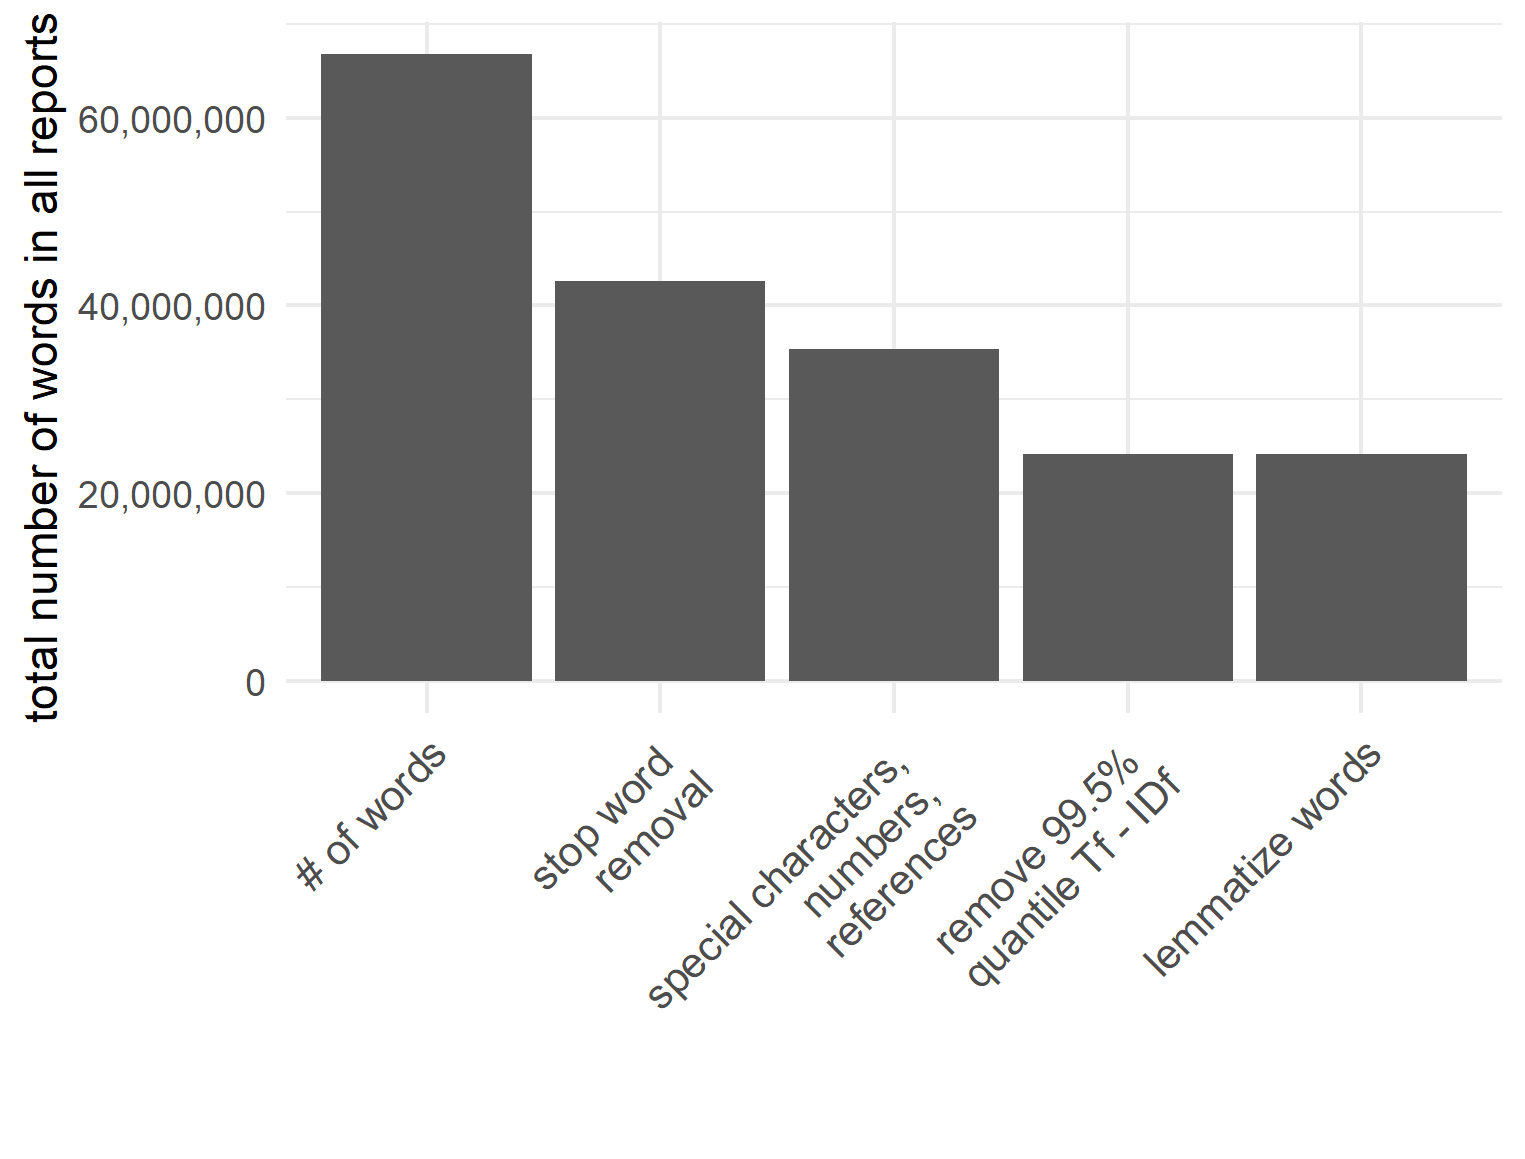
\includegraphics[width=\textwidth]{figures/ReductionInTotalNWords.png}
\caption{Reduction in total number of words due to preprocessing the data.}
\label{fig:TotWord}
\end{figure}

As explained earlier, the JST model is not good at dealing with words and topics which occur very frequently in one document, but not in any of the others. Those words that are too specific therefore have to be identified and removed. On way to do so is to look at the so called 'Term Frequency Inverse Document Frequency' (TF-IDF), which puts the feature frequency (FF) (also called term frequency (TF)) in relation to the inverse document frequency (IDF).
A high Term Frequency Inverse Document Frequency indicates that a word appears very often in one document but is very rare in others. The TF-IDF of a specific word in a certain document is calculated as:
\citep{na2004effectiveness}. 
\begin{equation}
    \text{TF-IDF} = \text{FF} * \log{\frac{\text{N}}{\text{DF}},}
\end{equation} 
where FF is the absolute number of occurrences of that word in the document, N represents the total number of documents in the text coprus, and DF is the number of documents in the corpus that contain the word. The result is a number between 0 and 1 for each word and document. For a large number of words, as in our case, TF-IDF values are usually quite low. For topic modelling like LDA the lower 10\% of words judged by TF-IDF are often removed, because they contain relatively frequent words over all documents. In our case however, the words to be removed contained relatively many adjectives relevant to sentiment extraction. We therefore did not remove the lower 10\% of words. We did, however, remove the highest ranked 0.05\% of words in every document as those are words very specific to this document, but very rare in others. Removing the 99.5 percent upper quantile of TF-IDF words seems indeed to improve the performance. An additional 10293 unique words were removed. The fourth and last step consists of lemmatizing the words using the \textit{textstem} package \citep{textstem}. Lemmatizing words means reducing them to their inflectional forms. The words 'are, is' are for example reduced to the word 'be'. After these four cleaning steps the number of individual words and items was reduced from 157380 to 64228 by about 60 Percent and of the total number of words only 36 Percent are left. The summary statistics for the total number of words in each report in Table \ref{tab:summaryCR} show the result more clearly. 
\begin{table}[ht]
\centering
\begin{tabular}{rllllll}
  \hline
  & Min. & 1st Qu. & Median  &  Mean & 3rd Qu. &   Max. \\
  \hline
  original reports & 16  &  1913  &  3230 &   3834  &  4785  & 21502  \\ 
  cleaned reports  & 0   &  729  &  1232  &  1400  &  1803  &  7218  \\ 
   \hline
\end{tabular}
\caption{Summary statistics for the number of words in each report. While originally the median report contained 3230 word we see it is now only a third of that.}
\label{tab:summaryCR}
\end{table}

\section{Sentiment Extraction - Results}\label{SentimentExtract}
In the following, we will present the results for the sentiment extraction performed with the sentiment library method and with JST. 

Figure \ref{fig:BoWSentiment} shows the distribution of the sentiment scores we obtained after using the document feature matrix \citep{quanteda} with the sentiment library in \texttt{R}. The polarity score was then calculated like in equation \ref{eq:polarity}. The histogram shows an approximate normal distribution around zero. This indicates that the sentiment extraction has worked and that the the imbalance in the number of positive ($n = 218$) and negative ($n = 1282)$) words does not affect the results negatively. 

\begin{figure}[h]
\centering
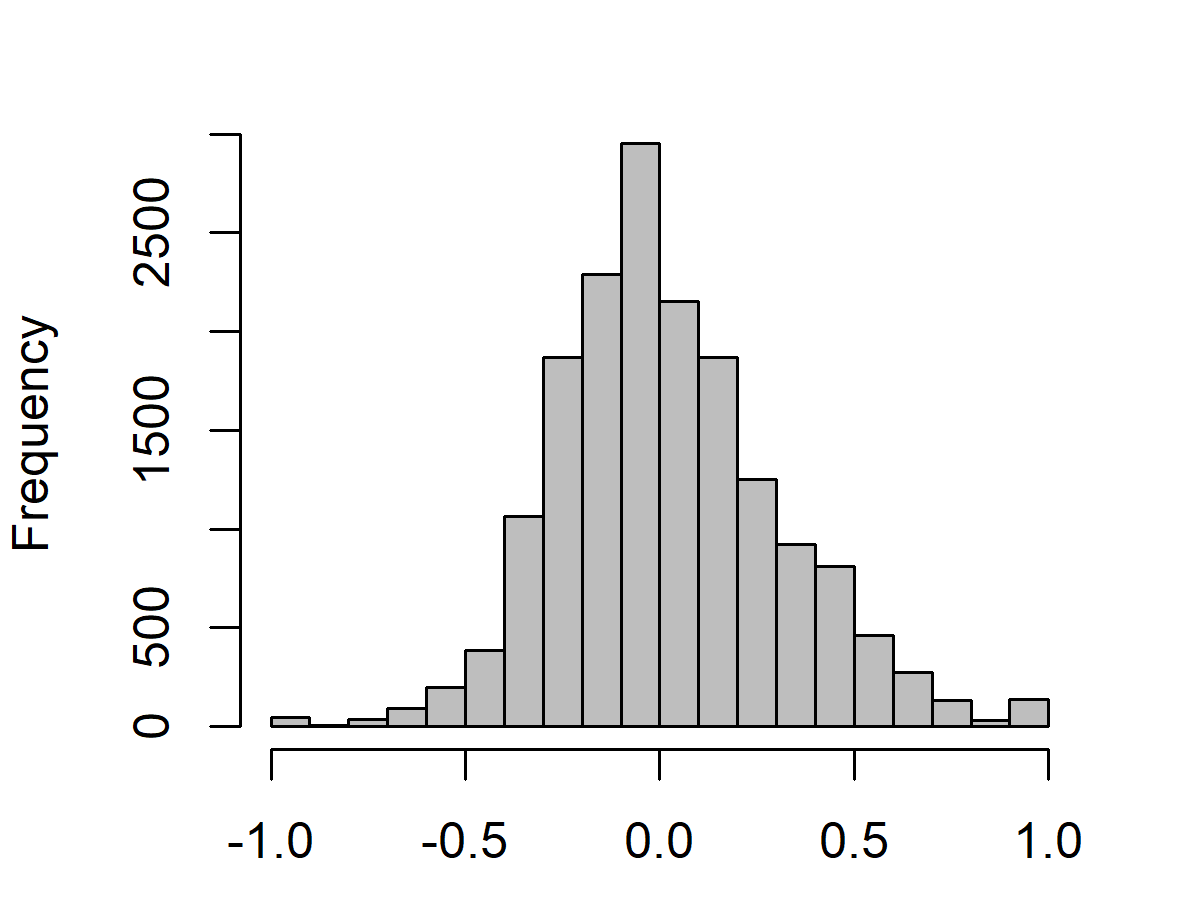
\includegraphics[width=4in]{figures/2SentimentsBOW_Histogram.png}
\caption{Histogram of the sentiment scores computed by the sentiment library}
\label{fig:BoWSentiment}
\end{figure}

The output of the JST models were generated using the \texttt{rJST} package in \texttt{R} \citep{rJST}. To improve the estimation, we have also added the sentiment dictionary used previously for the library method as prior information. From the model we obtained a set of posterior probabilities that link words, topics and documents together with sentiment scores. Based on a training data set that is large and diverse enough, those posterior probabilities can then be used to determine the topics and sentiment in a new document from the words used in them. 
\\
Because we do not have any labelled training data we cannot validate the results of the model externally, e.g. with the accuracy scores used in \citet{lin2009joint}. Instead we have to examine whether the association of words, topics, and sentiments proposed by the model look reasonable. We have always used two sentiments and tried different values for the number of topics to be estimated. We achieved the most reasonable results with 30 topics. Using the custom stop library as previously described and removing the top 0.05\% words as indicated by TF-IDF also improved the results. Due to the fact that we only have analyst reports for ten different stocks the results of the JST should still be regarded critically. 
Table \ref{tab:postProbSent1} gives an overview over the words  with the highest posterior probability for sentiment one on the topics one, two, three and thirty (see Table \ref{tab:postProbSent2}) in the appendix for sentiment. It is still visible that the documents come from a business context, but there are few words that directly indicate a sentiment like 'good', 'growth' and 'high'. This makes it hard to tell if the calculated sentiment one means positive, negative or something completely different. \\
% latex table generated in R 3.6.0 by xtable 1.8-4 package
% Fri Sep 13 15:15:05 2019
\begin{table}[ht]
\centering
\begin{tabular}{rlllll}
  \hline
 & topic1sent1 & topic2sent1 & topic3sent1 & \dots & topic30sent1 \\ 
  \hline
1 & good & year & customer & &price \\ 
  2 & look & margin & year & &volatility \\ 
  3 & company & will & service & &day \\ 
  4 & just & good & will & &stock \\ 
  5 & question & growth & business & &financial \\ 
  6 & mean & market & believe & &average \\ 
  7 & make & expect & continue & &expect \\ 
  8 & want & service & datum & &year \\ 
  9 & right & continue & growth & &next \\ 
  10 & business & high & line & &group \\ 
  11 & talk & next & fix & &express \\ 
  12 & people & single & also & &report \\ 
  13 & time & still & price & &month \\ 
  14 & content & also & industry & &rate \\ 
  15 & without & digit & time & &person \\ 
   \hline
\end{tabular}
\caption{Words for sentiment one with highest posterior probability per topic}
\label{tab:postProbSent1}
\end{table}
Another way to evaluate the model is to take a closer look at the posterior probabilities for the sentiments of all documents. The histogram in Figure \ref{fig:JSTSentiment} displays a split between a documents associated with sentiment 1 and others associated with sentiment 2. Note that with only two sentiments, the probabilities for a single document of belonging to sentiment 1 and to sentiment 2 add up to one. One could therefore obtain a histogram of sentiment 2 by mirroring this histogram at 0.5. The calculated sentiments clearly seem to lean towards the left, which indicates that sentiment two was more prominent in the data. \\
\begin{figure}[h]
\centering
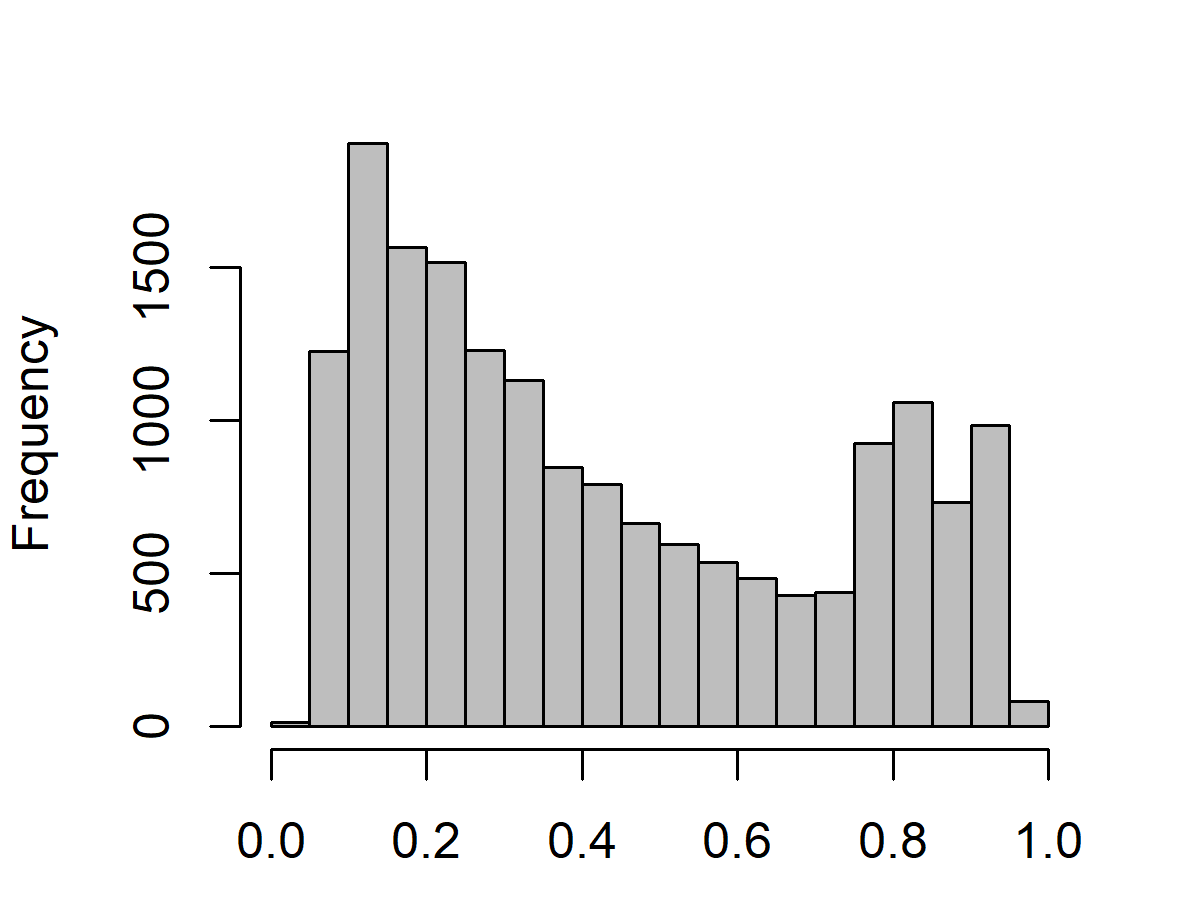
\includegraphics[width=4in]{figures/2SentimentsJST_Histogram.png}
\caption{Histogram of the sentiment scores computed by the Joined Sentiment Topic model}
\label{fig:JSTSentiment}
\end{figure}
The results of the unsupervised Joint Sentiment Models are difficult to evaluate and we have to be at least wary of the results we obtained. Problematic in this case could also be, that the JST views the documents as bag of words and therefore also ignores the ordering of words. Business language contains a lot of fixed phrases that are not considered here. Nonetheless they might be an informative feature for the estimation of stock price movements in the next section. 


\subsection{XG-Boost on sentiment data}\label{sec:XGB}
Based on the RavenPack data and our own custom sentiment scores we tried to make predictions for the movement of the time series of different stocks. Inspired by different Kaggle competitions and \citep{li2018predicting} we decided to try this using XGBoost for binary classification of upwards of downwards movement (which largely ignores the special time dependent structure of the data). XGBoost is a gradient tree boosting method developed by \citet{Chen_2016} and has several beneficial properties. Next to the computational properties it scales well for large data sets and can handle missing values internally. A possible competitor would be LightGBM by \citet{Ke2017LightGBMAH} from Microsoft. The general idea behind tree boosting is that they split data leaf-wise with the best fit, whereas other boosting algorithms split the tree level-wise. Splits are done only at the position where the loss can be reduced the most. The model creates an ensemble of a predefined number of classification and regression trees (CART) that complement each other. This tree ensemble method was originally developed by \citet{friedman2001greedy}. XGBoost which stands for "Extreme Gradient Boosting" can be seen as an extension of this framework. \\ \\
% good explanation: https://xgboost.readthedocs.io/en/latest/index.html
% mehr mathe?
%https://homes.cs.washington.edu/~tqchen/2016/03/10/story-and-lessons-behind-the-evolution-of-xgboost.html
After applying the two previously described sentiment extraction methods, we obtained one sentiment score from each model. For days where there existed multiple reports those scores we computed the average score and the standard deviation. The number of reports per day was also saved in another variable. In addition to the scores we included the log-returns of the previous day (logR yest) and current day (logR today) as well as the trading volume at that day (see Table \ref{tab:predictionFrame}). With this we are trying to predict a binary target, namely if the log-returns will be positive or negative the following day. Observations without corresponding analyst reports are omitted. 
From the RavenPack sentiment data we tried all the given variables together with "logR yest", "logR today" and "Volume". The RavenPack data has records for almost every day but some days have missing values when there was no sentiment recorded. Missing values are handled internally by XGBoost \citep{Chen_2016}. The model learns automatically where to go when a value is missing. For a large enough amount of data this is similar to imputing a value, but based on a reduction on training loss. 
\begin{table}[h]
\centering
\begin{tabular}{lrrrrrrr}
\toprule
{} &  logR today &  Volume &  logR yest. &  sent1 &  sentBoW &  sent1 sd &  \dots \\
utc\_date   &              &             &                     &             &               &           &                   \\
\midrule
2012-01-03 &       0.0000 &  45M &           0.0000 &      0.2790 &       -0.6190 &    0.0000 &         \dots \\
2012-01-04 &       0.0230 &  48M &              0.0000 &      0.7019 &        0.2318 &    0.1843 &      \dots \\
2012-01-05 &       0.0116 &  49M &              0.0230 &      0.1413 &        0.0000 &    0.0069 &      \dots \\
2012-01-06 &      -0.0060 &  36M &              0.0116 &      0.4749 &        0.1205 &    0.0257 &      \dots\\
2012-01-09 &       0.0090 &  47M &             -0.0060 &      0.6006 &       -0.6842 &    0.4526 &      \dots \\
2012-01-11 &       0.0084 &  57M &              0.0090 &      0.3607 &       -0.0296 &    0.2511 &      \dots \\
2012-01-12 &      -0.0020 &  44M &              0.0084 &      0.4279 &        0.0668 &    0.1181 &      \dots \\
2012-01-13 &      -0.0239 &  63M &             -0.0020 &      0.4603 &       -0.0076 &    0.2330 &      \dots \\
\bottomrule
\end{tabular}
    \caption{Excerpt from the data frame used for predictions}
    \label{tab:predictionFrame}
\end{table} 
The data was split into a training, validation and testing split by cutting the time series at predefined dates. Around 80 Percent where used for training and validation. Testing is done out of sample on values after 2016-12-10. For each stock, an independent model was fit and refitted after each prediction. After testing different hyper parameters we settled on a specification with 200 trees, a maximum depth of three, a learning rate of 0.05 and $\eta = 0.1$. Figure \ref{fig:tree} displays a random tree from the XGBoost tree ensemble for the RavenPack sentiment data. \\ 
\begin{figure}[h]
\centering
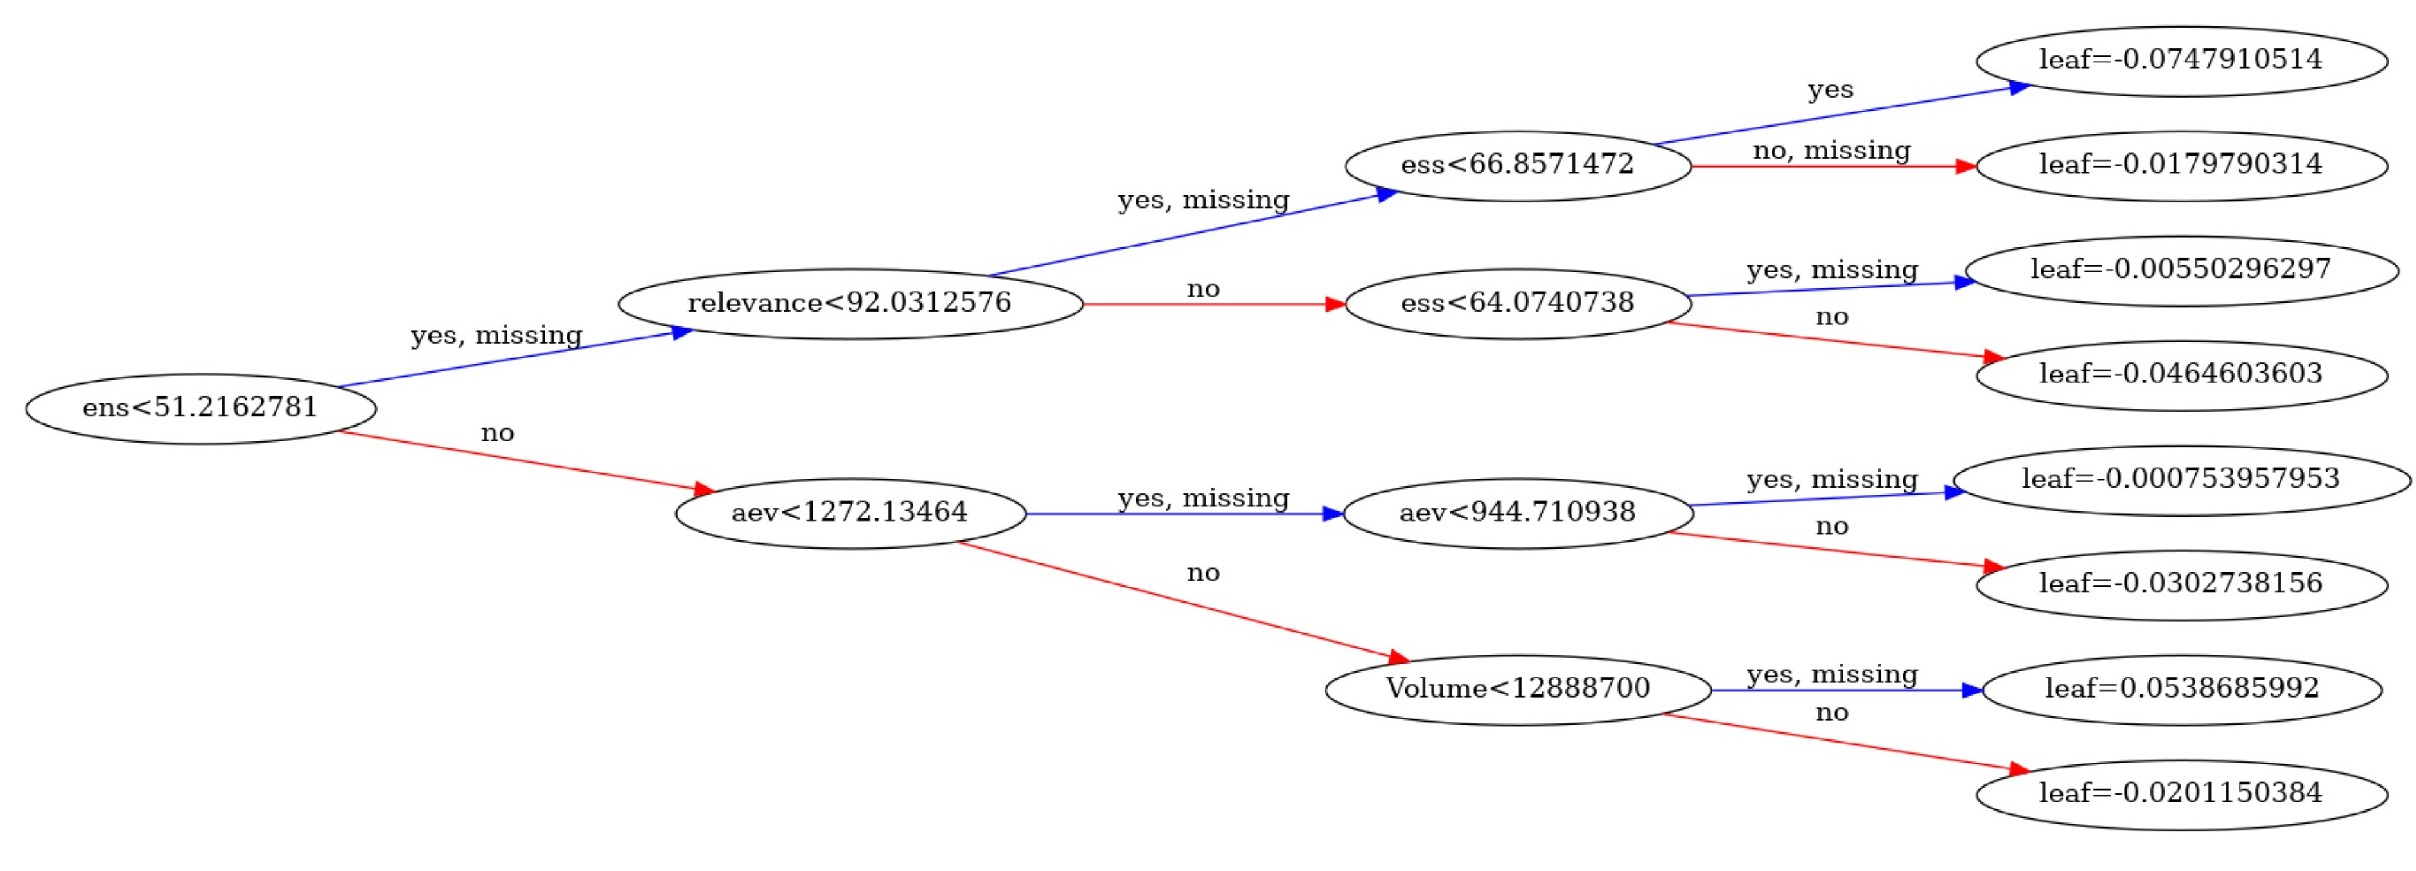
\includegraphics[width=\textwidth]{figures/treemodel2.jpg}
\caption{One of 200 random trees from the RavenPack tree ensemble}
\label{fig:tree}
\end{figure}

Even though we tried different hyper parameters, none seemed to make a large difference. Prediction accuracy was always around 50 Percent and the F1-measure (\ref{eq:f1score}) a standard evaluation metric of binary classification results \citep{HADDI201326} was consistently below 0.5.
\begin{equation} 
    \text{F1-measure} = \frac{2*\text{precision} * \text{recall}}{\text{precision} + \text{recall}}
\end{equation}\label{eq:f1score}
The results for the RavenPack data and our own sentiment scores can be found in Table \ref{tab:RavSentRes} and \ref{tab:OurSentRes}. By looking at the cross tables we also discovered that for some stocks class imbalances might cause the algorithm to mostly predict one class. 
\begin{table}[h]
\centering
\begin{tabular}{lrrrr}
\toprule
{} &  f1\_score &  accuracy &  precision &    recall \\
ticker &           &           &            &           \\
\midrule
MMM    &  0.3604 &  0.5849 &   0.5740 &  0.2627 \\
AXP    &  0.4100 &  0.5547 &   0.5061 &  0.3445 \\
GE     &  0.5932 &  0.4981 &   0.5574 &  0.6339 \\
INTC   &  0.4529 &  0.5169 &   0.4568 &  0.4491 \\
JNJ    &  0.4131 &  0.5283 &   0.5432 &  0.3333 \\
PG     &  0.5201 &  0.5056 &   0.4930 &  0.5503 \\
UTX    &  0.3236 &  0.5584 &   0.5090 &  0.2372 \\
VZ     &  0.4790 &  0.4830 &   0.5040 &  0.4565 \\
V      &  0.4549 &  0.5134 &   0.4308 &  0.4818 \\
DIS    &  0.3317 &  0.4830 &   0.4788 &  0.2537 \\
\midrule
mean & 0.4339 & 0.5226 & 0.5053 & 0.4003 \\
\bottomrule
\end{tabular}
    \caption{Prediction results for RavenPack sentiment data using XGBoost binary classification}
    \label{tab:RavSentRes}
\end{table}
%
\begin{table}[h]
\centering
\begin{tabular}{lrrrr}
\toprule
{} &  f1\_score &  accuracy &  precision &    recall \\
ticker &           &           &            &           \\
\midrule
MMM    &  0.2745 &  0.4788 &   0.4666 &  0.1944 \\
AXP    &  0.5263 &  0.4943 &   0.4385 &  0.6578 \\
GE     &  0.4836 &  0.4513 &   0.5606 &  0.4252 \\
INTC   &  0.3055 &  0.5575 &   0.3548 &  0.2682 \\
JNJ    &  0.2380 &  0.5362 &   0.4347 &  0.1639 \\
PG     &  0.4556 &  0.4487 &   0.4864 &  0.4285 \\
UTX    &  0.4556 &  0.4342 &   0.4000 &  0.5294 \\
VZ     &  0.4742 &  0.5142 &   0.5476 &  0.4181 \\
V      &  0.3437 &  0.4683 &   0.3548 &  0.3333 \\
DIS    &  0.4948 &  0.5663 &   0.6486 &  0.4000 \\
\midrule
mean &  0.4051 & 0.4949 & 0.4692 & 0.3818 \\
\bottomrule
\end{tabular}
    \caption{Prediction results for analyst reports sentiments using XGBoost binary classification}
    \label{tab:OurSentRes}
\end{table}
Variable importance plots can help to identify how important certain features are for the trees. As an example we illustrate the use based on the predictions for Disney. In Figure \ref{fig:VIP} the feature importance for the Disney RavenPack data is displayed on the left and the importance for the Disney sentiment scores is on the right. For the RavenPack data the estimated novelty score loads the highest followed by the number of events over a 90 day period. For the sentiment data from the analyst reports trading volume and the two sentiment scores contain the most information according to the model. Over the course of trying different model specifications the sentiment score from the library method reliably outperformed the Joint Sentiment Topic model. The standard deviation of the JST sentiment scores seems to confer no meaning at all for the model. These visual results need to be treated with care, because the model precision appears to be relatively poor. It would have been interesting to obtain a probability or certainty score together with the prediction. Unfortunately, this is not possible with XGBoost. Overall, our results are similar to the ones reported e.g. by \citet{atkins2018financial} in that our prediction accuracy is usually lower than 50 Percent. 

\begin{figure}[h!]
    \centering
    \figuretitle{Feature Importance Plots}
    \begin{adjustbox}{width=.95\textwidth,center}
        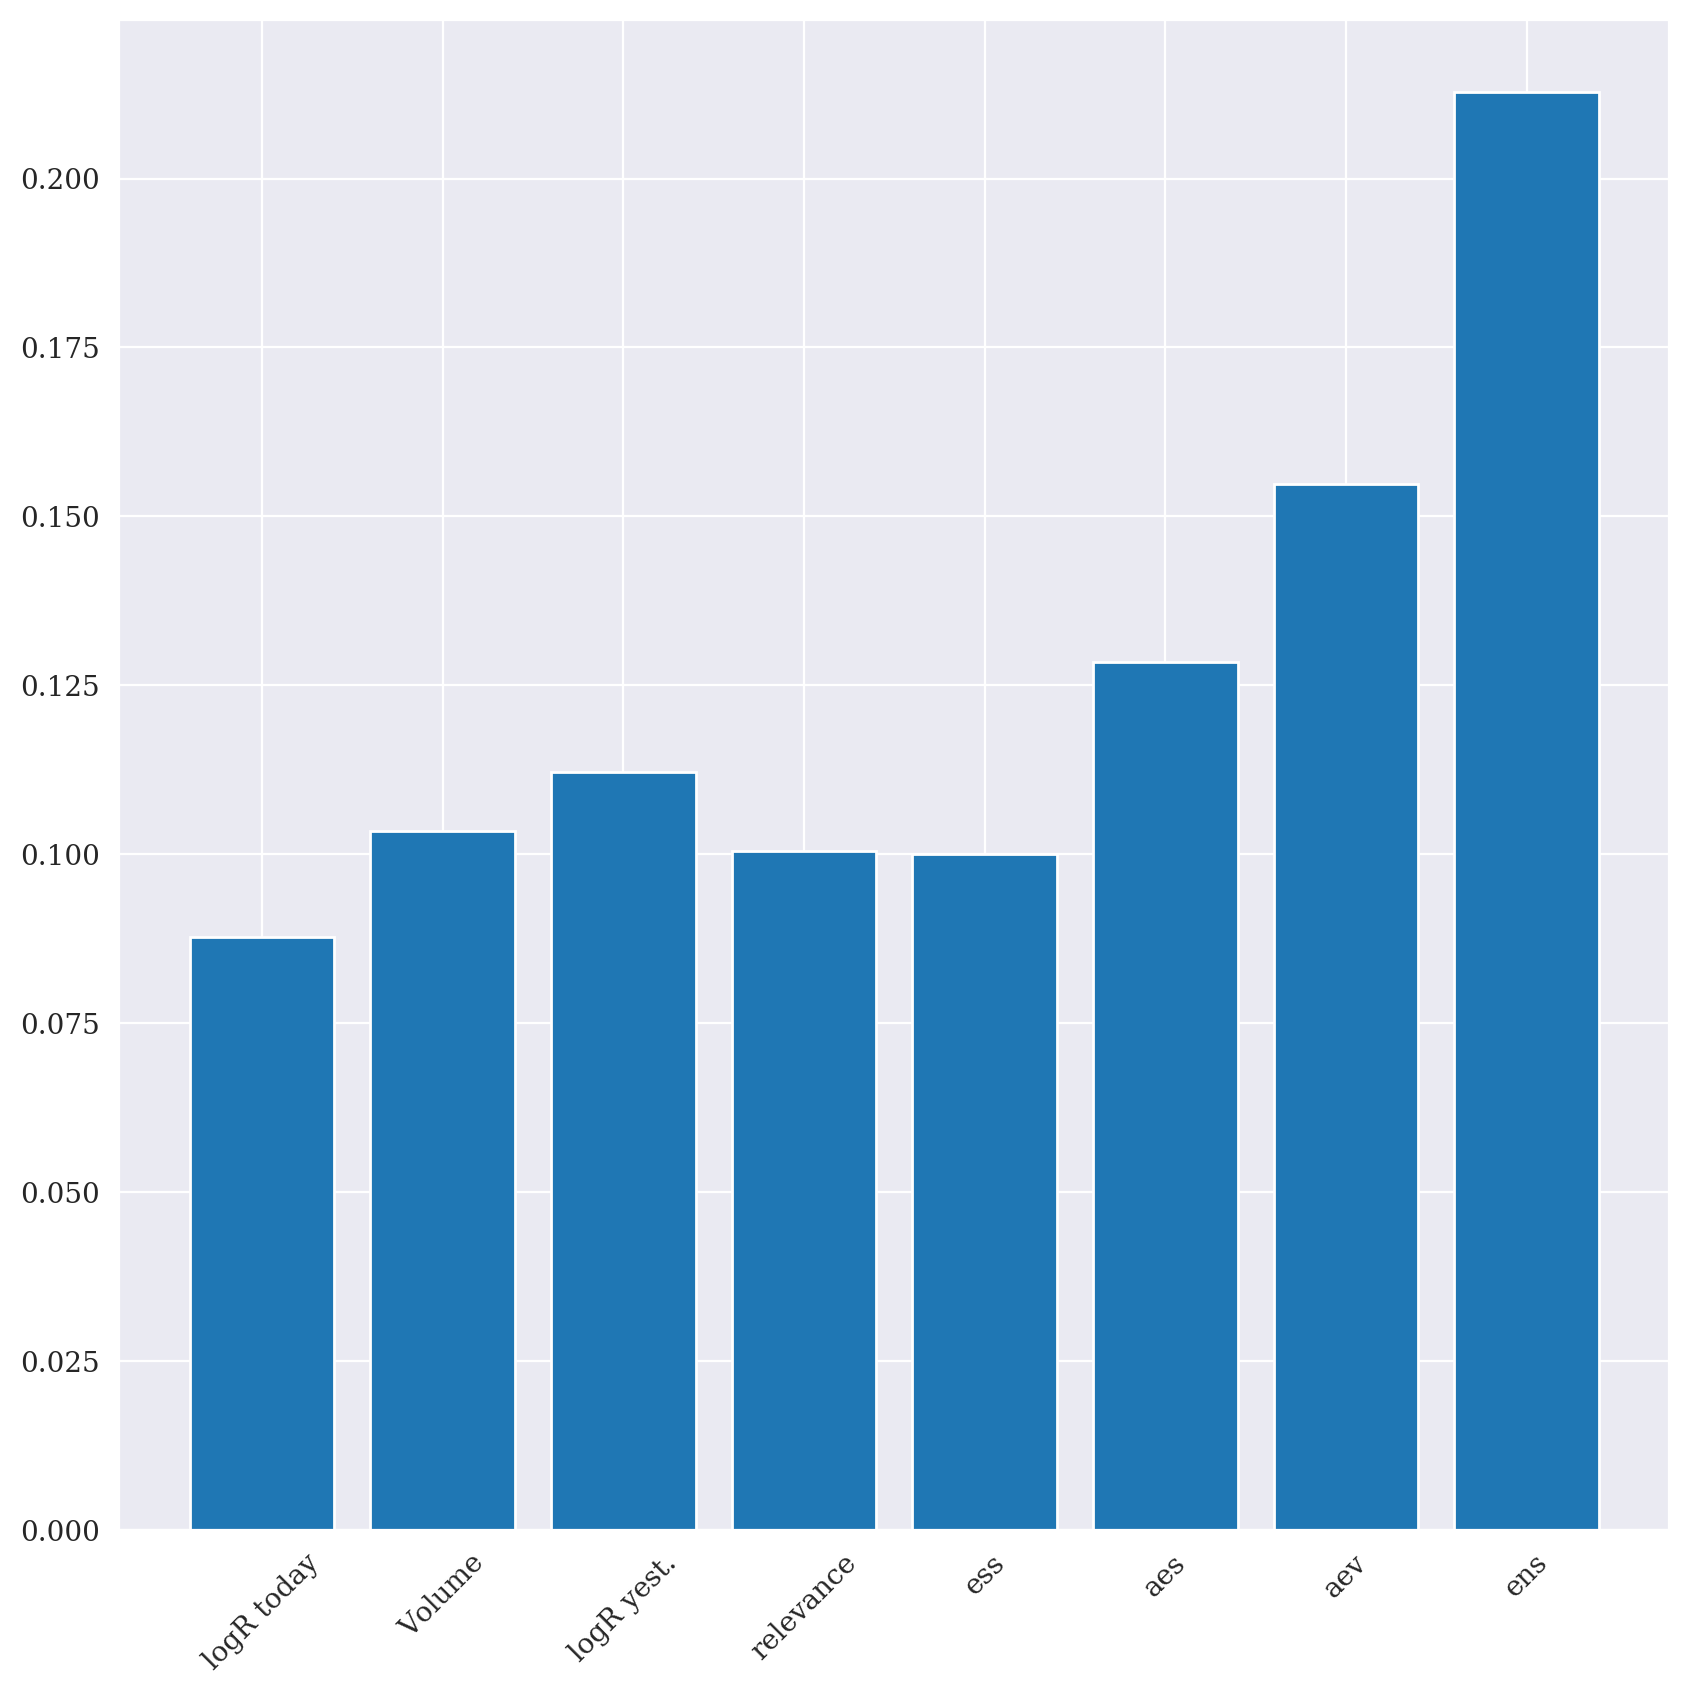
\includegraphics[width = \linewidth]{figures/XGBoostRav_tomorrow_iterative.png}
        %\input{figures/XGBoostRav_tomorrow_iterative.png}
        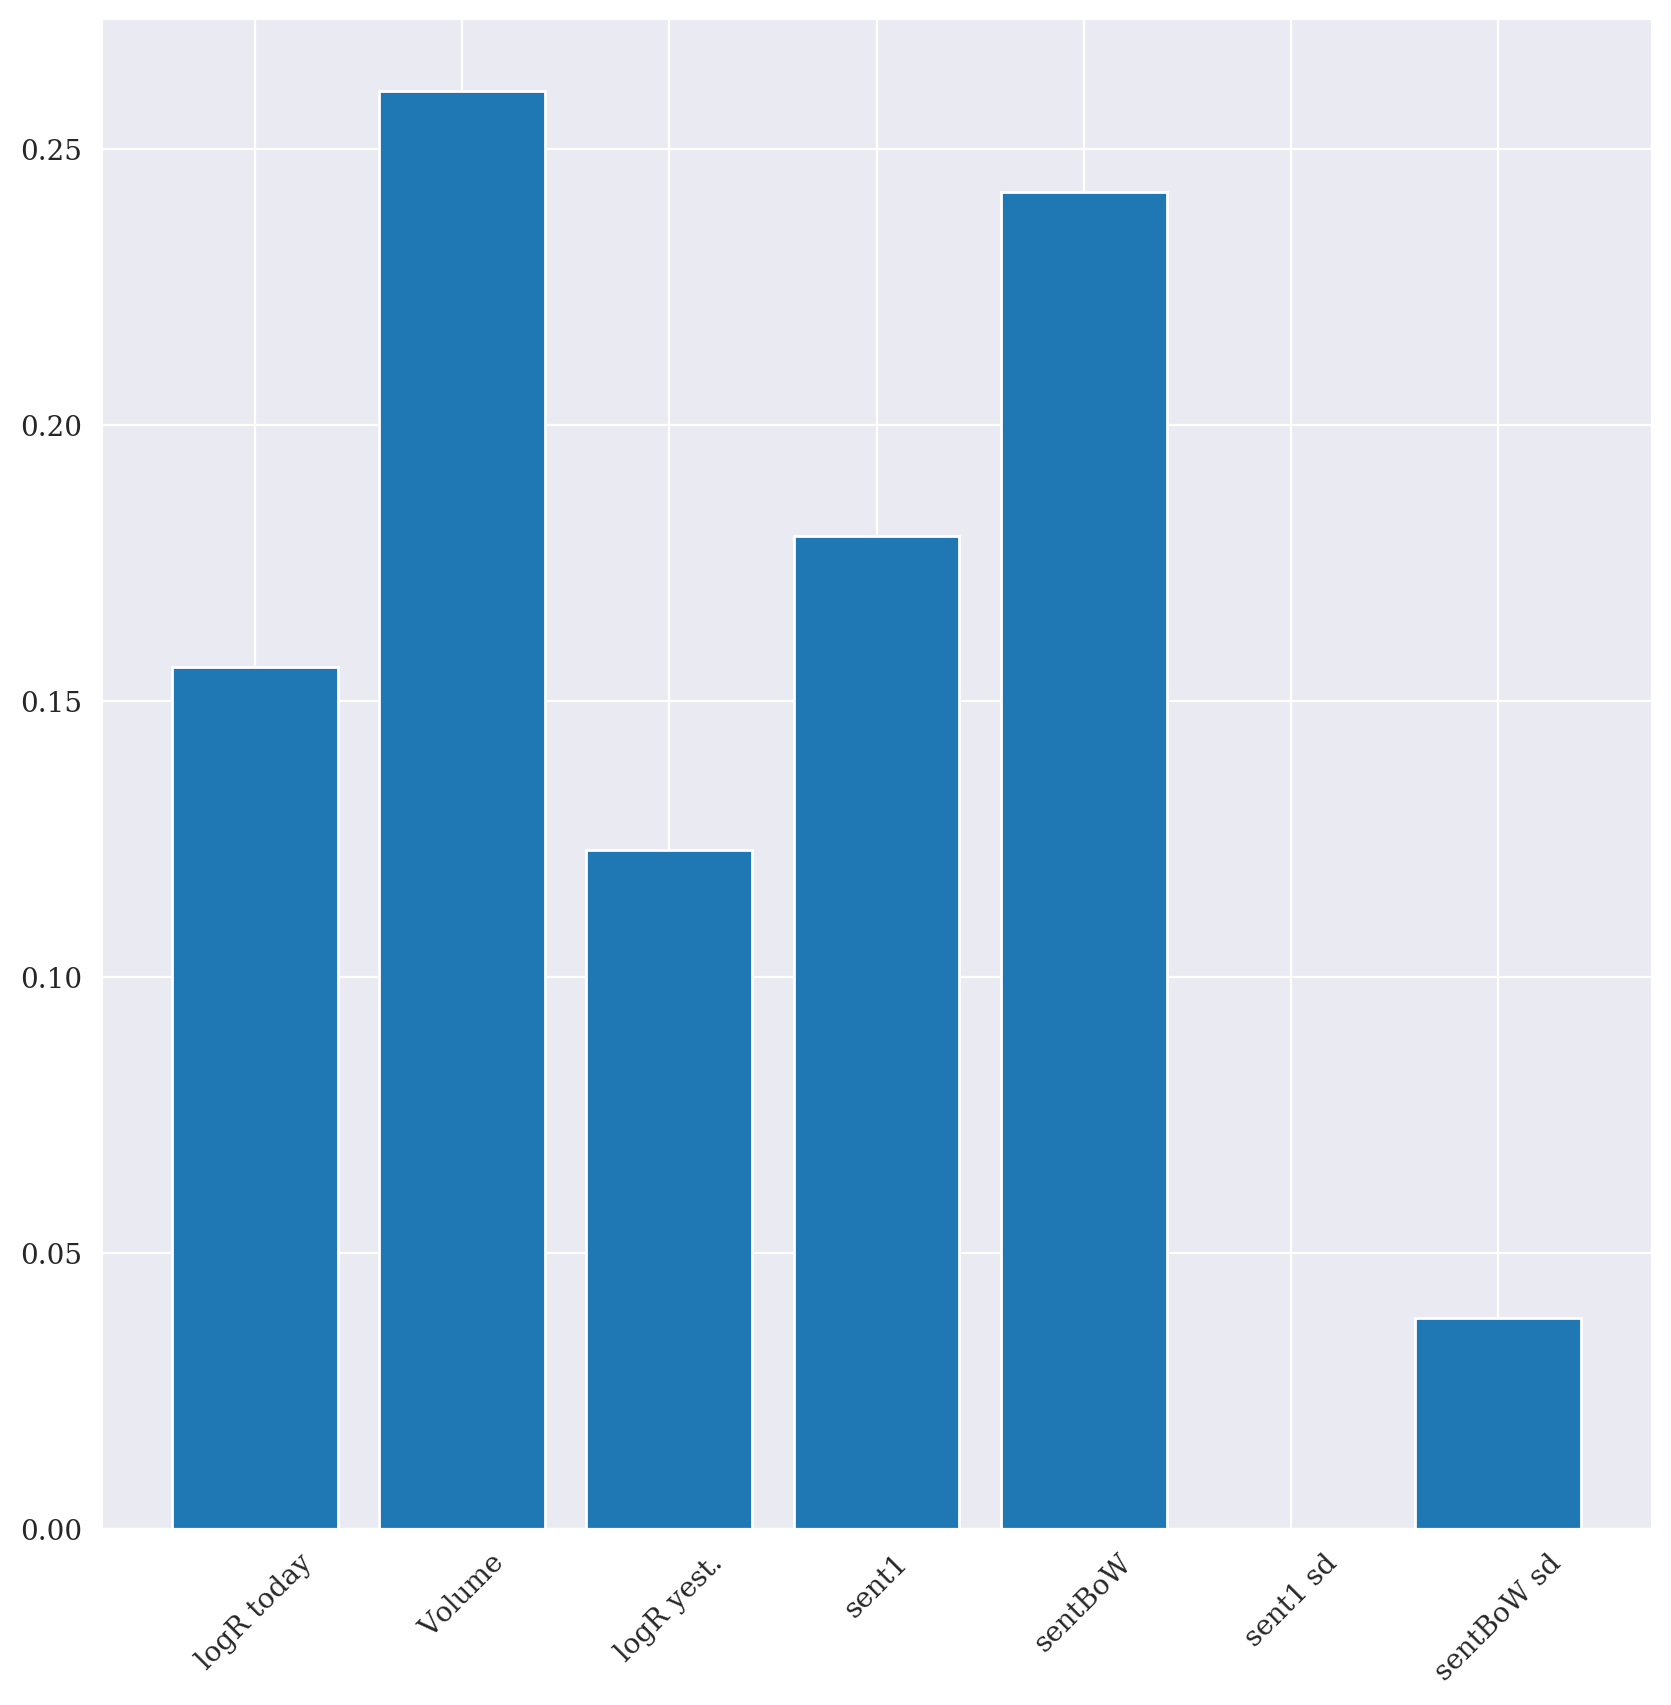
\includegraphics[width = \linewidth]{figures/XGBoostSent_tomorrow_iterative.png}
        %\input{figures/XGBoostSent_tomorrow_iterative.png}
    \end{adjustbox}  
    \caption{On the left the feature importance plot for Disney RavenPack model and on the right the corresponding one for the Disney analyst reports.}
    \label{fig:VIP}
\end{figure}
%What would have also be interesting would be to model market uncertainty and volatility as opposed to the movement of the time series itself. 



